\begin{figure}[htbp]
\begin{subfigure}{0.72\textwidth}
    \begin{tikzpicture}
    [x=0.06667\textwidth, y=0.06667\textwidth]
    \draw (0,0) rectangle (15,7);
    % chamber
    \draw[fill=vacuum]
        (.5,1.5) rectangle (3.5,6.5);
    \draw[fill=gold]
        (1.7,1.95)--
        (2.3,1.95)--
        (2.3,1.8)--
        (1.7,1.8)--
        (1.7,1.95);
    \draw[fill=darkgrey]
        (1,2.1)--
        (1.65,2.1)--
        (1.75,1.8)--
        (2.25,1.8)--
        (2.35,2.1)--
        (3,2.1)--
        (3,2)--
        (2.4,2)--
        (2.3,1.7)--
        (1.7,1.7)--
        (1.6,2)--
        (1,2)--
        (1,2.1);
    \draw[gold,dashed,line width=0.003\textwidth]
        (2,2) -- (2,5);
    \coordinate (a) at (2,5);
    \def\theta{20}
    \draw[fill=darkgrey,rotate=\theta,shift={(a)}]
        (-1,-.1) rectangle (1,.1);
    \draw[angle,dotted,line width=0.003\textwidth,rotate=\theta,shift={(a)}]
        (0,-.1) -- (0,-1.5);
    \draw[angle,line width=0.002\textwidth,shift={(a)}]
        (0,-1.2) arc(270:270+\theta:1.2);
    \draw[fill=substrate,rotate=\theta,shift={(a)}]
        (-.2,-.1) rectangle (.2,.-.2)
        (-.8,-.1) rectangle (-.4,.-.2)
        (.4,-.1) rectangle (.8,.-.2);
    \draw[fill=sphere,rotate=\theta,shift={(a)}]
        (-.2,-.2) rectangle (.2,.-.22)
        (-.8,-.2) rectangle (-.4,.-.22)
        (.4,-.2) rectangle (.8,.-.22);
    \draw[omega,line width=0.01\textwidth,rotate=\theta,shift={(a)}]
        (0,.1) -- (0,1.2);
    \draw[omega,<->,line width=0.003\textwidth,rotate=\theta,shift={(a)}]
        (0,.4)++(120:.5) arc(120:420:.5 and .15);
    % zoom
    \coordinate (sp1) at ($(a)+(\theta:.6)+.16*(sin{\theta},-cos{\theta})$);
    \coordinate (sp2) at (5.5,3.85);
    \draw[spy,line width=0.002\textwidth]
        (sp1) circle(.25)
        (sp2) circle(1.9)
        ($(sp1)+(90:.25)$)--($(sp2)+(100:1.9)$)
        ($(sp1)+(230:.25)$)--($(sp2)+(220:1.9)$);
    \coordinate (s) at (4,1);
    \draw[fill=substrate,shift={(s)}]
        (0.5,4.1) rectangle (2.5,4.3)
        (0.5,1.5) rectangle (2.5,3.5);
    \foreach \i in {1.63,1.9764,...,3.41}
        \foreach \j in {0.6,0.8,...,2.41}
            \filldraw[sphere,shift={(s)}] (\j,\i) circle (0.105);
    \foreach \i in {1.8032,2.1496,...,3.41}
        \foreach \j in {0.7,0.9,...,2.41}
            \filldraw[sphere,shift={(s)}] (\j,\i) circle (0.105);
    \foreach \i in {0.6,0.8,...,2.41}
        \filldraw[sphere,shift={(s)}]
            (\i,4.01) ellipse [x radius=0.105,y radius=0.09];
    % second zoom
    \coordinate (sp3) at (6.1,2.9);
    \coordinate (sp4) at (7.7,1.3);
    \draw[spy,line width=0.002\textwidth]
        (sp3) circle(.25)
        (sp4) circle(1.2)
        ($(sp3)+(60:.25)$)--($(sp4)+(70:1.2)$)
        ($(sp3)+(210:.25)$)--($(sp4)+(194:1.2)$);
    \filldraw[sphere,shift={($(sp4)-(0,0.148)$)}]
        (-.5,0.433) circle(.525)
        (.5,0.433) circle(.525)
        (0,-0.433) circle(.525);
    % cross section
    \coordinate (m) at (12,2.5);
    \def\shift{1.2}
    \coordinate (lda) at
        ($
        (m)
        +(-\shift,0.6)
        +(cos{\theta},0)
        -(1/cos{\theta}*sin{\theta},0)
        +(sin{\theta}*sin{\theta}/cos{\theta},0)
        $);
    \coordinate (ldb) at
        ($
        (m)
        +(-\shift,3.5)
        +(cos{\theta},0)
        +(2.9/cos{\theta}*sin{\theta},0)
        -(1/cos{\theta}*sin{\theta},0)
        +(sin{\theta}*sin{\theta}/cos{\theta},0)
        $);
    \coordinate (rua) at
        ($
        (m)
        +(+\shift,0.6)
        -(cos{\theta},0)
        -(1/cos{\theta}*sin{\theta},0)
        -(sin{\theta}*sin{\theta}/cos{\theta},0)
        $);
    \coordinate (rub) at
        ($
        (m)
        +(+\shift,3.5)
        -(cos{\theta},0)
        +(2.9/cos{\theta}*sin{\theta},0)
        -(1/cos{\theta}*sin{\theta},0)
        -(sin{\theta}*sin{\theta}/cos{\theta},0)
        $);
    \draw[goldray,fill=gold,fill opacity=0.3,line width=0.003\textwidth]
        (lda)--(ldb)--
        (rub)--(rua)--
        (lda);
    \filldraw[gold]
        (lda)rectangle($(rua)+(0,0.08)$);
    \coordinate (rda) at
        ($
        (m)
        +(\shift,0.6)
        -(cos{\theta},0)
        +(1/cos{\theta}*sin{\theta},0)
        -(sin{\theta}*sin{\theta}/cos{\theta},0)
        $);
    \coordinate (rdb) at
        ($
        (m)
        +(\shift,3.5)
        -(cos{\theta},0)
        -(2.9/cos{\theta}*sin{\theta},0)
        +(1/cos{\theta}*sin{\theta},0)
        -(sin{\theta}*sin{\theta}/cos{\theta},0)
        $);
    \coordinate (lua) at
        ($
        (m)
        +(-\shift,0.6)
        +(cos{\theta},0)
        +(1/cos{\theta}*sin{\theta},0)
        +(sin{\theta}*sin{\theta}/cos{\theta},0)
        $);
    \coordinate (lub) at
        ($
        (m)
        +(-\shift,3.5)
        +(cos{\theta},0)
        -(2.9/cos{\theta}*sin{\theta},0)
        +(1/cos{\theta}*sin{\theta},0)
        +(sin{\theta}*sin{\theta}/cos{\theta},0)
        $);
    \draw[goldray,fill=gold,opacity=0.8,fill opacity=0.1,dashed,line width=0.003\textwidth]
        (rda)--(rdb)--
        (lub)--(lua)--
        (rda);
    \filldraw[gold]
        (rda)rectangle($(lua)+(0,0.08)$);
    \draw[crosssection,dotted,line width=0.003\textwidth,shift={(sp4)}]
        (-1.2,0)--(1.2,0);
    \draw[crosssection,line width=0.003\textwidth,shift={(m)}]
        (-2.5,0)rectangle(2.5,3.5);
    \draw[crosssection,line width=0.002\textwidth]
        (sp4)++(1.2,0)--($(m)+(-2.5,2)$);
    \filldraw[sphere,shift={(m)}]
        (\shift,1.6) circle(1)
        (-\shift,1.6) circle(1);
    \draw[fill=substrate,shift={(m)}]
        (-2.3,0.2)rectangle(2.3,.6);
    \draw[omega,<->,line width=0.002\textwidth,shift={(m)}]
        (0,2.9)++(120:.55) arc(120:420:.55 and .1);
    \draw[angle,dashed,line width=0.003\textwidth,shift={(m)}]
        (0,0.6)--(0,3.5);
    \coordinate (rellda) at ($(m)-(lda)+(0,0.6)$);
    \ExtractCoordinate{rellda}
    \coordinate (point) at ($(m)+(0,\XCoord/sin{\theta}*cos{\theta})$);
    \draw[angle,line width=0.002\textwidth]
        ($(point)+(0,0.9)+(0,0.6)$) arc(90:90-\theta:0.9);
    % split-ring
    \draw[split,shift=(m)]
        (-0.8,0.4)rectangle(0.8,0.8)
        (0,0.4)--(0,-0.2);
    \draw[split,fill=substrate,shift=(m)]
        (-0.8,-0.2)rectangle(0.8,-1.8);
    \coordinate (O) at ($(m)-(0,1)$);
    \coordinate (split1) at (\XCoord,0);
    \coordinate (relrua) at ($(m)-(rua)+(0,0.6)$);
    \ExtractCoordinate{relrua}
    \coordinate (split) at ($(split1)+(0,\XCoord)$);
    \ExtractCoordinate{split}
    \draw[fill=gold]
        (O)++(-55:\XCoord)
        arc(-55:235:\XCoord)
        --($(O)+(235:\YCoord)$)
        arc(235:-55:\YCoord)
        --($(O)+(-55:\XCoord)$);
    \end{tikzpicture}
    \subcaption{evaporation}
\end{subfigure}
\hfill
\begin{subfigure}{0.26\textwidth}
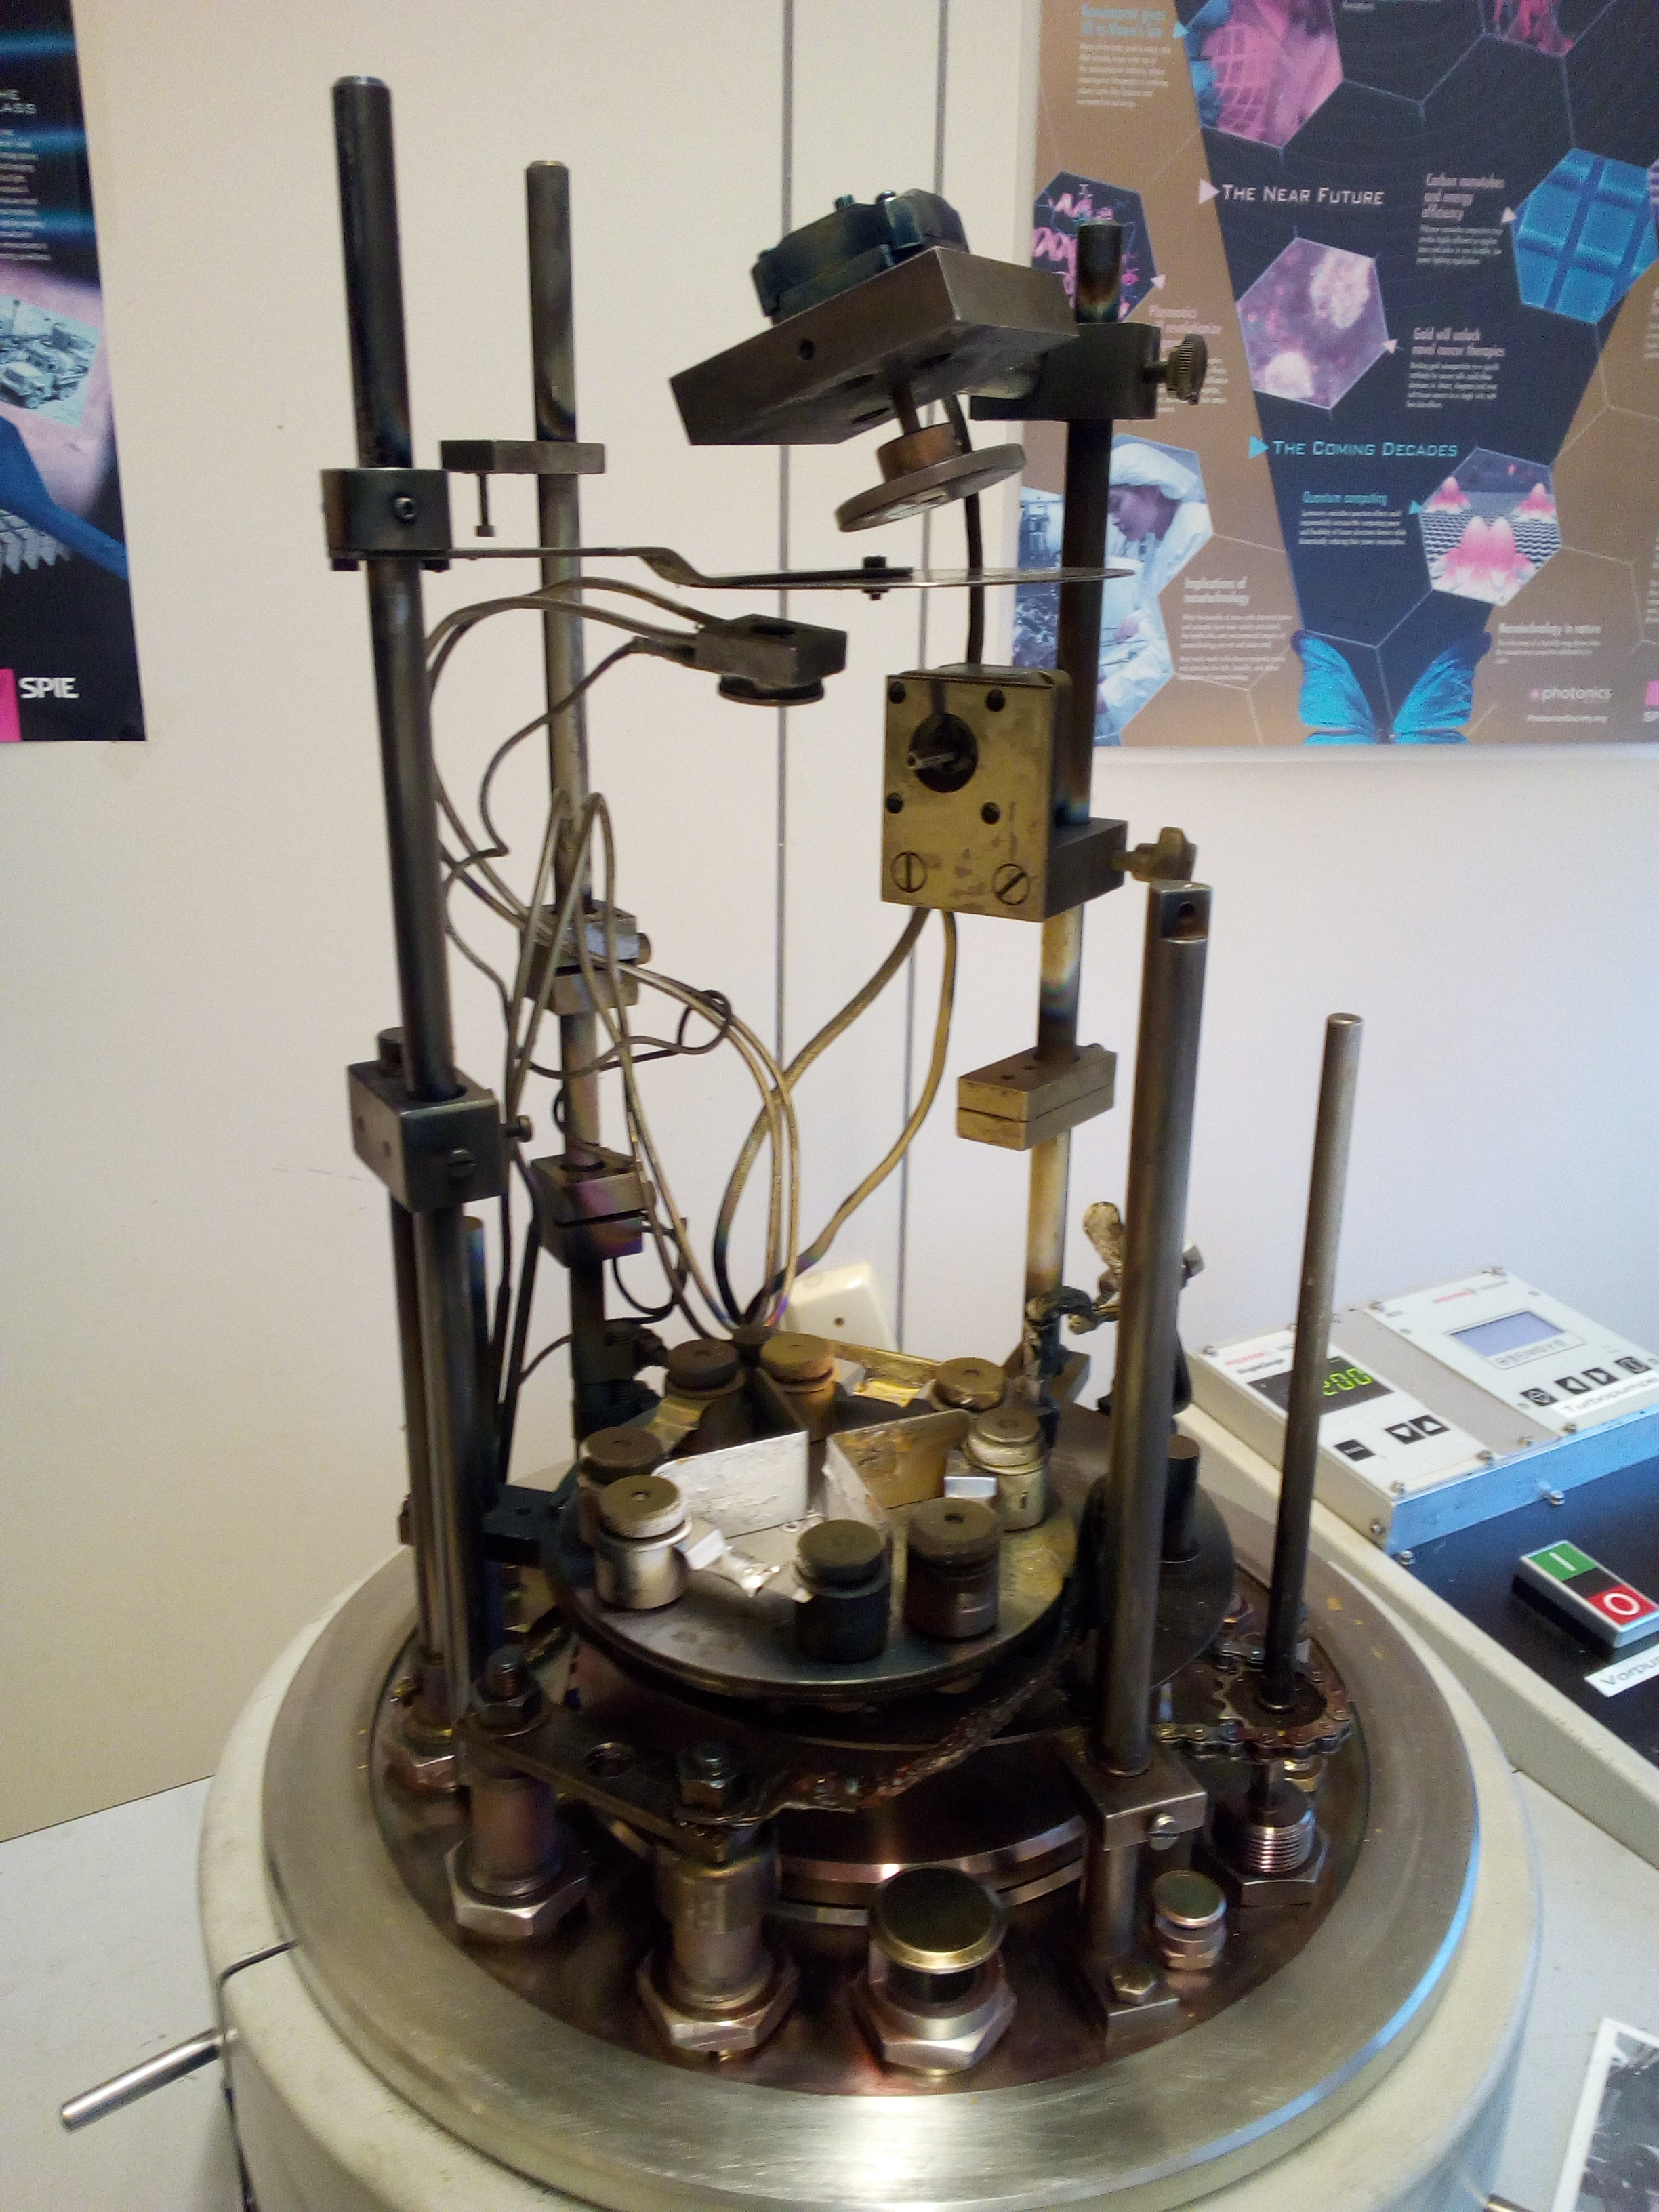
\includegraphics[width=\textwidth]{chamber.jpg}
\subcaption{evaporation chamber}
\end{subfigure}
\end{figure}